\chapter[Revisão teórica]{Revisão teórica} \label{cap:cap1}
    Colocar texto aqui 
    
    \section{Sistemas Multirrobô} \label{sec:mrs}
        Colocar texto aqui
    
        \subsection{Taxonomias} \label{subsec:taxonomias_mrs}
    
    \section{Alocação de Tarefas em Sistema Multirrobô} \label{sec:mrta}
        Um dos problemas mais desafiadores em aplicações multi-robôs é denominado como \textit{alocação de tarefas}, (MRTA, acrônimo para \textit{Multi-Robot Task Allocation}). Problemas dessa natureza buscam como solução atribuir otimamente um conjunto de robôs para um conjunto de tarefas de maneira que o desempenho geral de um sistema sujeito a um conjunto de limitações seja otimizado.
        
        \textcolor{red}{falar sobre o conteúdo desta seção}
        
        
        \subsection{Definição Formal} \label{subsec:mrta_formal}
    
        \subsection{Taxonomias} \label{subsec:taxonomia_mrta}
            \citeonline{ref:gerkey2004taxonomy} sugeriram uma taxonomia de três eixos independente do domínio de para a classificação de problemas de alocação de tarefas em sistemas multi-robôs. 
            
            O primeiro eixo determina o \textit{tipo dos robôs} que compõem o problema. Os tipos de robôs possíveis são: \textit{ST} (acrônimo para \textit{Single-Task}) ou \textit{MT} (acrônimo para \textit{Multi-Task}). Problemas que envolvem robôs que só podem executar uma tarefa por vez são compostos por robôs do tipo \textit{ST}. Entretanto, se houver pelo menos um robô capaz de executar mais de uma tarefa simultaneamente, então esse problema é composto por robôs do tipo \textit{MT}. 
            
            O segundo eixo da taxonomia determina o \textit{tipo das tarefas} que compõem o problema. Nesse caso, são possíveis os tipos: \textit{ST} (acrônimo para \textit{Single-Robot}) ou \textit{MR} (acrônimo para \textit{Multi-Robot}). Problemas cujo tipo das tarefas é \textit{SR}, diz-se que todas as tarefas envolvidas só podem ser executadas por um robô. Porém, quando o tipo das tarefas envolvidas é \textit{MR}, diz-se que existe tarefas que podem ser executadas por mais de um robô.
            
            O terceiro eixo, por sua vez, determina o \textit{tipo da alocação} do problema, o qual pode assumir os valores: \textit{IA} (acrônimo para \textit{Instantaneous Assignment}) ou \textit{TA} (acrônimo para \textit{Time-extended Assignment}). O primeiro caso, \textit{IA}, diz repeito à problemas MRTA onde as alocações das tarefas para os robôs são realizadas instantaneamente, sem levar em consideração o estado futuro do sistema. Por outro lado, em problemas cujo tipo de alocação é \textit{TA}, além de conhecido o estado atual de cada rôbo e do ambiente, também é conhecido o conjunto de tarefas que precisarão ser alocadas no futuro. Neste último caso, diversas tarefas são alocadas para um robô, o qual deve executar cada alocação conforme seu agendamento. De acordo com \cite{ref:bastos2008utility}, quando o tipo de alocação do problema MRTA é \textit{IA}, o número de robôs é superior ao número de tarefas alocadas e quando \textit{TA}, o oposto acontece. Isso se deve ao fato de que, em problemas MRTA cujo tipo de alocação é \textit{IA}, o número de robôs no sistema é capaz de suprir a taxa de tarefas a serem atribuídas, de modo que é muito provável que haverão robôs ociosos no sistema; enquanto, naqueles cujo tipo de alocação é \textit{TA}, o número de robôs que compõem o sistema não é suficiente para atender a taxa de tarefas a serem alocadas no sistema.
            
            \begin{figure}[htb]
                \centering
                % Graphic for TeX using PGF
% Title: ../figures/taxonomia_mrta.dia
% Creator: Dia v0.97.2
% CreationDate: Tue Oct 17 17:33:09 2017
% For: adrianohrl
% \usepackage{tikz}
% The following commands are not supported in PSTricks at present
% We define them conditionally, so when they are implemented,
% this pgf file will use them.
\ifx\du\undefined
  \newlength{\du}
\fi
\setlength{\du}{15\unitlength}
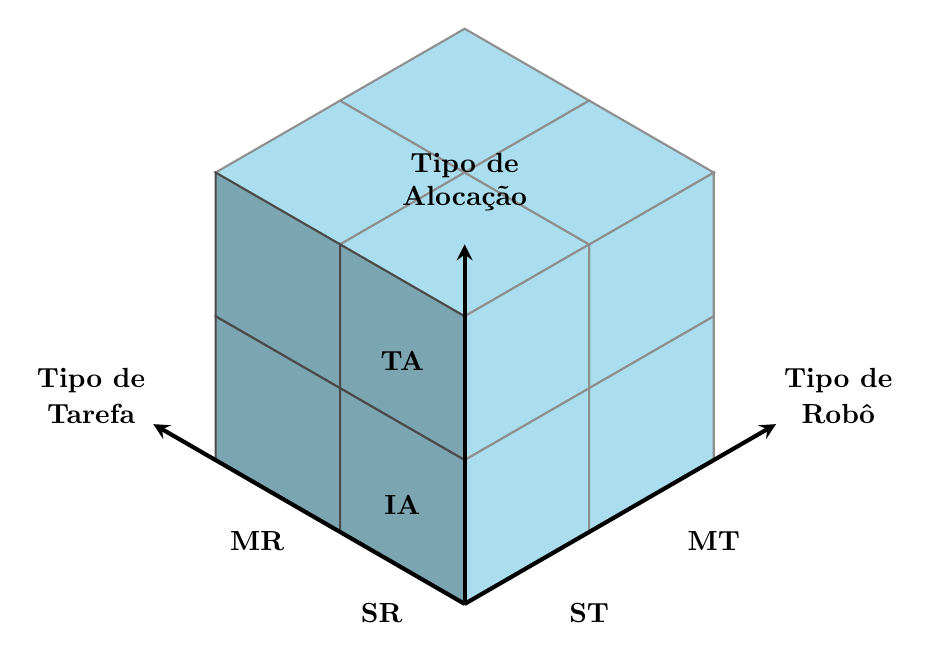
\begin{tikzpicture}
\pgftransformxscale{1.000000}
\pgftransformyscale{-1.000000}
\definecolor{dialinecolor}{rgb}{0.000000, 0.000000, 0.000000}
\pgfsetstrokecolor{dialinecolor}
\definecolor{dialinecolor}{rgb}{1.000000, 1.000000, 1.000000}
\pgfsetfillcolor{dialinecolor}
\pgfsetlinewidth{0.050000\du}
\pgfsetdash{}{0pt}
\pgfsetdash{}{0pt}
\pgfsetmiterjoin
\pgfsetbuttcap
\definecolor{dialinecolor}{rgb}{0.666667, 0.870588, 0.937255}
\pgfsetfillcolor{dialinecolor}
\fill (-5.500000\du,-10.392300\du)--(-2.500000\du,-8.660250\du)--(0.500000\du,-10.392300\du)--(-2.500000\du,-12.124400\du)--cycle;
\definecolor{dialinecolor}{rgb}{0.556863, 0.556863, 0.556863}
\pgfsetstrokecolor{dialinecolor}
\draw (-5.500000\du,-10.392300\du)--(-2.500000\du,-8.660250\du)--(0.500000\du,-10.392300\du)--(-2.500000\du,-12.124400\du)--cycle;
\pgfsetlinewidth{0.050000\du}
\pgfsetdash{}{0pt}
\pgfsetdash{}{0pt}
\pgfsetmiterjoin
\pgfsetbuttcap
\definecolor{dialinecolor}{rgb}{0.666667, 0.870588, 0.937255}
\pgfsetfillcolor{dialinecolor}
\fill (-2.500000\du,-12.124400\du)--(0.500000\du,-10.392300\du)--(3.500000\du,-12.124400\du)--(0.500000\du,-13.856400\du)--cycle;
\definecolor{dialinecolor}{rgb}{0.556863, 0.556863, 0.556863}
\pgfsetstrokecolor{dialinecolor}
\draw (-2.500000\du,-12.124400\du)--(0.500000\du,-10.392300\du)--(3.500000\du,-12.124400\du)--(0.500000\du,-13.856400\du)--cycle;
\pgfsetlinewidth{0.050000\du}
\pgfsetdash{}{0pt}
\pgfsetdash{}{0pt}
\pgfsetmiterjoin
\pgfsetbuttcap
\definecolor{dialinecolor}{rgb}{0.666667, 0.870588, 0.937255}
\pgfsetfillcolor{dialinecolor}
\fill (3.500000\du,-8.660250\du)--(3.500000\du,-5.196150\du)--(6.500000\du,-6.928200\du)--(6.500000\du,-10.392300\du)--cycle;
\definecolor{dialinecolor}{rgb}{0.556863, 0.556863, 0.556863}
\pgfsetstrokecolor{dialinecolor}
\draw (3.500000\du,-8.660250\du)--(3.500000\du,-5.196150\du)--(6.500000\du,-6.928200\du)--(6.500000\du,-10.392300\du)--cycle;
\pgfsetlinewidth{0.050000\du}
\pgfsetdash{}{0pt}
\pgfsetdash{}{0pt}
\pgfsetmiterjoin
\pgfsetbuttcap
\definecolor{dialinecolor}{rgb}{0.666667, 0.870588, 0.937255}
\pgfsetfillcolor{dialinecolor}
\fill (-2.500000\du,-8.660250\du)--(0.500000\du,-6.928200\du)--(3.500000\du,-8.660250\du)--(0.500000\du,-10.392300\du)--cycle;
\definecolor{dialinecolor}{rgb}{0.556863, 0.556863, 0.556863}
\pgfsetstrokecolor{dialinecolor}
\draw (-2.500000\du,-8.660250\du)--(0.500000\du,-6.928200\du)--(3.500000\du,-8.660250\du)--(0.500000\du,-10.392300\du)--cycle;
\pgfsetlinewidth{0.050000\du}
\pgfsetdash{}{0pt}
\pgfsetdash{}{0pt}
\pgfsetmiterjoin
\pgfsetbuttcap
\definecolor{dialinecolor}{rgb}{0.666667, 0.870588, 0.937255}
\pgfsetfillcolor{dialinecolor}
\fill (0.500000\du,-10.392300\du)--(3.500000\du,-8.660250\du)--(6.500000\du,-10.392300\du)--(3.500000\du,-12.124400\du)--cycle;
\definecolor{dialinecolor}{rgb}{0.556863, 0.556863, 0.556863}
\pgfsetstrokecolor{dialinecolor}
\draw (0.500000\du,-10.392300\du)--(3.500000\du,-8.660250\du)--(6.500000\du,-10.392300\du)--(3.500000\du,-12.124400\du)--cycle;
\pgfsetlinewidth{0.050000\du}
\pgfsetdash{}{0pt}
\pgfsetdash{}{0pt}
\pgfsetmiterjoin
\pgfsetbuttcap
\definecolor{dialinecolor}{rgb}{0.666667, 0.870588, 0.937255}
\pgfsetfillcolor{dialinecolor}
\fill (0.500000\du,-6.928200\du)--(0.500000\du,-3.464100\du)--(3.500000\du,-5.196150\du)--(3.500000\du,-8.660250\du)--cycle;
\definecolor{dialinecolor}{rgb}{0.556863, 0.556863, 0.556863}
\pgfsetstrokecolor{dialinecolor}
\draw (0.500000\du,-6.928200\du)--(0.500000\du,-3.464100\du)--(3.500000\du,-5.196150\du)--(3.500000\du,-8.660250\du)--cycle;
\pgfsetlinewidth{0.050000\du}
\pgfsetdash{}{0pt}
\pgfsetdash{}{0pt}
\pgfsetmiterjoin
\pgfsetbuttcap
\definecolor{dialinecolor}{rgb}{0.666667, 0.870588, 0.937255}
\pgfsetfillcolor{dialinecolor}
\fill (0.500000\du,-3.464100\du)--(0.500000\du,0.000000\du)--(3.500000\du,-1.732050\du)--(3.500000\du,-5.196150\du)--cycle;
\definecolor{dialinecolor}{rgb}{0.556863, 0.556863, 0.556863}
\pgfsetstrokecolor{dialinecolor}
\draw (0.500000\du,-3.464100\du)--(0.500000\du,0.000000\du)--(3.500000\du,-1.732050\du)--(3.500000\du,-5.196150\du)--cycle;
\pgfsetlinewidth{0.050000\du}
\pgfsetdash{}{0pt}
\pgfsetdash{}{0pt}
\pgfsetmiterjoin
\pgfsetbuttcap
\definecolor{dialinecolor}{rgb}{0.666667, 0.870588, 0.937255}
\pgfsetfillcolor{dialinecolor}
\fill (3.500000\du,-5.196150\du)--(3.500000\du,-1.732050\du)--(6.500000\du,-3.464100\du)--(6.500000\du,-6.928200\du)--cycle;
\definecolor{dialinecolor}{rgb}{0.556863, 0.556863, 0.556863}
\pgfsetstrokecolor{dialinecolor}
\draw (3.500000\du,-5.196150\du)--(3.500000\du,-1.732050\du)--(6.500000\du,-3.464100\du)--(6.500000\du,-6.928200\du)--cycle;
\pgfsetlinewidth{0.050000\du}
\pgfsetdash{}{0pt}
\pgfsetdash{}{0pt}
\pgfsetmiterjoin
\pgfsetbuttcap
\definecolor{dialinecolor}{rgb}{0.486275, 0.647059, 0.698039}
\pgfsetfillcolor{dialinecolor}
\fill (-2.500000\du,-8.660250\du)--(-2.500000\du,-5.196150\du)--(-5.500000\du,-6.928200\du)--(-5.500000\du,-10.392300\du)--cycle;
\definecolor{dialinecolor}{rgb}{0.290196, 0.290196, 0.290196}
\pgfsetstrokecolor{dialinecolor}
\draw (-2.500000\du,-8.660250\du)--(-2.500000\du,-5.196150\du)--(-5.500000\du,-6.928200\du)--(-5.500000\du,-10.392300\du)--cycle;
\pgfsetlinewidth{0.050000\du}
\pgfsetdash{}{0pt}
\pgfsetdash{}{0pt}
\pgfsetmiterjoin
\pgfsetbuttcap
\definecolor{dialinecolor}{rgb}{0.486275, 0.647059, 0.698039}
\pgfsetfillcolor{dialinecolor}
\fill (0.500000\du,-6.928200\du)--(0.500000\du,-3.464100\du)--(-2.500000\du,-5.196150\du)--(-2.500000\du,-8.660250\du)--cycle;
\definecolor{dialinecolor}{rgb}{0.290196, 0.290196, 0.290196}
\pgfsetstrokecolor{dialinecolor}
\draw (0.500000\du,-6.928200\du)--(0.500000\du,-3.464100\du)--(-2.500000\du,-5.196150\du)--(-2.500000\du,-8.660250\du)--cycle;
\pgfsetlinewidth{0.050000\du}
\pgfsetdash{}{0pt}
\pgfsetdash{}{0pt}
\pgfsetmiterjoin
\pgfsetbuttcap
\definecolor{dialinecolor}{rgb}{0.486275, 0.647059, 0.698039}
\pgfsetfillcolor{dialinecolor}
\fill (-2.500000\du,-5.196150\du)--(-2.500000\du,-1.732050\du)--(-5.500000\du,-3.464100\du)--(-5.500000\du,-6.928200\du)--cycle;
\definecolor{dialinecolor}{rgb}{0.290196, 0.290196, 0.290196}
\pgfsetstrokecolor{dialinecolor}
\draw (-2.500000\du,-5.196150\du)--(-2.500000\du,-1.732050\du)--(-5.500000\du,-3.464100\du)--(-5.500000\du,-6.928200\du)--cycle;
\pgfsetlinewidth{0.050000\du}
\pgfsetdash{}{0pt}
\pgfsetdash{}{0pt}
\pgfsetmiterjoin
\pgfsetbuttcap
\definecolor{dialinecolor}{rgb}{0.486275, 0.647059, 0.698039}
\pgfsetfillcolor{dialinecolor}
\fill (0.500000\du,-3.464100\du)--(0.500000\du,0.000000\du)--(-2.500000\du,-1.732050\du)--(-2.500000\du,-5.196150\du)--cycle;
\definecolor{dialinecolor}{rgb}{0.290196, 0.290196, 0.290196}
\pgfsetstrokecolor{dialinecolor}
\draw (0.500000\du,-3.464100\du)--(0.500000\du,0.000000\du)--(-2.500000\du,-1.732050\du)--(-2.500000\du,-5.196150\du)--cycle;
% setfont left to latex
\definecolor{dialinecolor}{rgb}{0.000000, 0.000000, 0.000000}
\pgfsetstrokecolor{dialinecolor}
\node at (-8.500000\du,-5.374900\du){\textbf{Tipo de}};
% setfont left to latex
\definecolor{dialinecolor}{rgb}{0.000000, 0.000000, 0.000000}
\pgfsetstrokecolor{dialinecolor}
\node at (-8.500000\du,-4.574900\du){\textbf{Tarefa}};
% setfont left to latex
\definecolor{dialinecolor}{rgb}{0.000000, 0.000000, 0.000000}
\pgfsetstrokecolor{dialinecolor}
\node at (0.500000\du,-10.571050\du){\textbf{Tipo de}};
% setfont left to latex
\definecolor{dialinecolor}{rgb}{0.000000, 0.000000, 0.000000}
\pgfsetstrokecolor{dialinecolor}
\node at (0.500000\du,-9.771050\du){\textbf{Alocação}};
% setfont left to latex
\definecolor{dialinecolor}{rgb}{0.000000, 0.000000, 0.000000}
\pgfsetstrokecolor{dialinecolor}
\node at (9.500000\du,-5.374900\du){\textbf{Tipo de}};
% setfont left to latex
\definecolor{dialinecolor}{rgb}{0.000000, 0.000000, 0.000000}
\pgfsetstrokecolor{dialinecolor}
\node at (9.500000\du,-4.574900\du){\textbf{Robô}};
\pgfsetlinewidth{0.100000\du}
\pgfsetdash{}{0pt}
\pgfsetdash{}{0pt}
\pgfsetbuttcap
{
\definecolor{dialinecolor}{rgb}{0.000000, 0.000000, 0.000000}
\pgfsetfillcolor{dialinecolor}
% was here!!!
\pgfsetarrowsstart{stealth}
\definecolor{dialinecolor}{rgb}{0.000000, 0.000000, 0.000000}
\pgfsetstrokecolor{dialinecolor}
\draw (8.000000\du,-4.330130\du)--(0.500000\du,0.000000\du);
}
\pgfsetlinewidth{0.100000\du}
\pgfsetdash{}{0pt}
\pgfsetdash{}{0pt}
\pgfsetbuttcap
{
\definecolor{dialinecolor}{rgb}{0.000000, 0.000000, 0.000000}
\pgfsetfillcolor{dialinecolor}
% was here!!!
\pgfsetarrowsstart{stealth}
\definecolor{dialinecolor}{rgb}{0.000000, 0.000000, 0.000000}
\pgfsetstrokecolor{dialinecolor}
\draw (-7.000000\du,-4.330130\du)--(0.500000\du,0.000000\du);
}
% setfont left to latex
\definecolor{dialinecolor}{rgb}{0.000000, 0.000000, 0.000000}
\pgfsetstrokecolor{dialinecolor}
\node at (-4.500000\du,-1.510800\du){\textbf{MR}};
% setfont left to latex
\definecolor{dialinecolor}{rgb}{0.000000, 0.000000, 0.000000}
\pgfsetstrokecolor{dialinecolor}
\node at (-1.500000\du,0.221250\du){\textbf{SR}};
% setfont left to latex
\definecolor{dialinecolor}{rgb}{0.000000, 0.000000, 0.000000}
\pgfsetstrokecolor{dialinecolor}
\node at (3.500000\du,0.221250\du){\textbf{ST}};
% setfont left to latex
\definecolor{dialinecolor}{rgb}{0.000000, 0.000000, 0.000000}
\pgfsetstrokecolor{dialinecolor}
\node at (6.500000\du,-1.510800\du){\textbf{MT}};
% setfont left to latex
\definecolor{dialinecolor}{rgb}{0.000000, 0.000000, 0.000000}
\pgfsetstrokecolor{dialinecolor}
\node at (-1.000000\du,-5.840930\du){\textbf{TA}};
% setfont left to latex
\definecolor{dialinecolor}{rgb}{0.000000, 0.000000, 0.000000}
\pgfsetstrokecolor{dialinecolor}
\node at (-1.000000\du,-2.376830\du){\textbf{IA}};
\pgfsetlinewidth{0.100000\du}
\pgfsetdash{}{0pt}
\pgfsetdash{}{0pt}
\pgfsetbuttcap
{
\definecolor{dialinecolor}{rgb}{0.000000, 0.000000, 0.000000}
\pgfsetfillcolor{dialinecolor}
% was here!!!
\pgfsetarrowsstart{stealth}
\definecolor{dialinecolor}{rgb}{0.000000, 0.000000, 0.000000}
\pgfsetstrokecolor{dialinecolor}
\draw (0.500000\du,-8.660250\du)--(0.500000\du,0.000000\du);
}
\end{tikzpicture}

                \caption[Representação visual da taxonomia de três eixos]{Representação visual da taxonomia de três eixos sugerida por \citeonline{ref:gerkey2004taxonomy}.} \label{fig:taxomia_mrta}
            \end{figure}
            
            É visto na Figura \ref{fig:taxomia_mrta} uma representação gráfica da taxonomia de \cite{ref:gerkey2004taxonomy} para a classificação de problemas MRTA (\textit{Multi-Robot Task Allocation}), onde pode-se notar que existem oito classes de problemas MRTA bem definidos.
            
            \emph{\color{red} dar exemplo}
            
            \textbf{\color{red} Uma nova taxonomia foi sugerida por ...}
            
            \emph{\color{red} definir o escopo de problemas considerados neste trabalho}
            
        \subsubsection{Arquiteturas MRTA} \label{subsec:arquiteturas_mrta}
            Possuem a função de solucionar problemas de alocação de tarefas em sistemas mutirrobô.
        
            \subsection{Arquiteturas baseadas em Comportamento} \label{subsec:arch_comportamento}
            
            \begin{itemize}
                \item \textbf{ALLIANCE}: \cite{ref:parker1998alliance};
                \item \textbf{L-ALLIANCE}: \cite{ref:parker1996lalliance};
                
            \end{itemize}
            
            \subsection{Arquiteturas baseadas em Mercado} \label{subsec:arch_mercado}
    
            \begin{itemize}
                \item \textbf{Murdoch}: \cite{ref:gerkey2002murdoch};
                \item \textbf{M+}: \cite{ref:botelho1999m+};
                
            \end{itemize}
                
    \section{ROS}
        Acrônimo para \textit{Robot Operating System} \cite{ref:quigley2009ros}, o ROS é uma \textit{framework} para robótica que tem incentivado a comunidade de pesquisadores em robótica a trabalhar conjuntamente desde seu lançamento.
    
        Primeiramente, ROS é flexível. Um projeto atômico baseado em ROS, denominado pacote, pode ser desenvolvido em diversas linguagens de programação. Deste modo, seus desenvolvedores podem tirar proveito das vantagens que cada linguagem suportada tem, sejam elas eficiência em tempo de execução, confiabilidade, recursos, síntaxe, semântica ou documentação existente. Atualmente, as linguagens de programação suportadas são C++, Python e Lisp. As linguagens Java e Lua ainda estão em fase de desenvolvimento.
        
        Projetos de robótica possuem rotinas que poderia ser reutilizadas em outros projetos. Por esta razão, ROS é também modular, pois pacotes configuráveis existentes podem ser combinados para realizar uma aplicação especifica. Várias bibliotecas externas já foram adaptadas para ser usadas no ROS: aruco\footnote{\url{http://wiki.ros.org/ar_sys}}, gmapping\footnote{\url{http://wiki.ros.org/gmapping}}, interfaces de programação para aplicações de robôs\footnote{\url{http://wiki.ros.org/Robots}}, sensores\footnote{\url{http://wiki.ros.org/Sensors}} e simuladores\footnote{\url{http://wiki.ros.org/gazebo}}, planejadores\footnote{\url{http://kcl-planning.github.io/ROSPlan/}}, reconhecimento de voz\footnote{\url{http://wiki.ros.org/Sensors\#Audio_.2BAC8_Speech_Recognition}}, entre outros. Isso evidencia que os usuários de ROS podem focar no desenvolvimento de pesquisa de sua área e contribuir da melhor forma com essa comunidade.
        
        Em adição, ROS disponibiliza diversas ferramentas para auxiliar no desenvolvimento de projetos e, também, verificar o funcionamento de aplicação. Suas ferramentas típicas são: \textit{get} e \textit{set} de parâmetros de configuração, vizualização da topologia de conexão \textit{peer-to-peer}, medição de utilização de banda, gráficos dos dados de mensagem e outras mais. É altamente recomendado o uso dessas ferramentas para garantir a estabilidade e confiança dos pacotes desenvolvidos, que normalmente têm alta complexidade.
        
        Uma lacuna que antes existia na nova geração de aplicações robóticas foi preenchida com o lançamento do ROS. Como um fornecedor de serviços de \textit{middleware}, ele (1) simplifica o desenvolvimento de processos, (2) suporta comunicação e interoperabilidade, (3) oferece e facilita serviços frequentemente utilizados em robótica e, ainda, oferece (4) utilização eficiente dos seus recursos disponíveis, (5) abstrações heterogênicas e (6) descoberta e configuração automática de recursos \cite{ref:quigley2009ros}. No intuito de cobrir todas exigências de um \textit{middleware}, ROS 2.0 tenta dar suporte à sistemas embarcados e dispositivos de baixo recurso.
        
        Como resultado, 
        
        Over the years, it has been noticed that:
    	(1) the number of contributors (academic researchers and industry) and projects have increased;
    	(2) the applications have became more sophisticated;
    	(3) the degree of difficulty of solved problems has ??? in different areas of robotics field;
    	(4) the robotic industry has been more interested to contribute.
    	
    	\textcolor{red}{citar exemplo de middlewares para robótica}
        
        \textcolor{red}{falar sobre o conteúdo deste capítulo}
        
        \subsection{Conceitos Básicos} \label{sec:ros_conceitos}
        
            Sua concepção foi baseada em conceitos divididos em três níveis: (1) Sistema de Arquivos do ROS, (2) Grafo de Computação do ROS e (3) Comunidade do ROS. A seguir será explicado cada um desses níveis, cada um com seu respectivo conjunto de conceitos. Além disso, também serão detalhados os dois tipos de nomes definidos no ROS: nomes de recursos de pacote e nomes de recursos de grafo.
            
            \subsubsection{Sistema de Arquivos do ROS}
                
                Os conceitos envolvidos no nível do \textit{Sistema de Arquivos do ROS} se referem aos arquivos armazenados em disco. São eles:
                
                \begin{itemize}
                    \item \textbf{Pacotes}: em inglês \textit{Packages}, é uma forma atômica de organização de criação e lançamento de \textit{software} no ROS. Um pacote contém definições de processos (nós), de dependência de bibliotecas, de tipos de mensagens, ações e serviços, de estruturas de dados e, por fim, de configuração. 
                    
                    \item \textbf{Meta-Pacotes}: em inglês \textit{Metapackages}, é um tipo especial de pacote que tem por objetivo agrupar pacotes relacionados.
                    
                    \item \textbf{Manifestos de Pacote}: em inglês \textit{Package Manifests}, arquivo nomeado \textit{package.xml} contido na raíz de cada pacote. Seu papel é fornecer meta-informações sobre seu pacote: nome, versão, descrição, informações de licença, dependências, entre outras. 
                    
                    \item \textbf{Tipos de Mensagem}: em inglês \textit{Message Types}, arquivos de extensão \textit{.msg}, localizados dentro da pasta \textit{msg} de um dado pacote. Seu conteúdo define a estrutura de dados de uma mensagem que poderá ser enviado pelo ROS.
                    
                    \item \textbf{Tipos de Serviço}: em inglês \textit{Service Types}, arquivos de extensão \textit{.srv}, localizados dentro da pasta \textit{srv} de um dado pacote. Seu conteúdo define a estrutura de dados das mensagens de requisito e resposta de um serviço, as quais poderão ser enviadas pelo ROS.
                \end{itemize}
            
            \subsubsection{Grafo de Computação do ROS}
        
                O \textit{Grafo de Computação do ROS} é uma rede ponto-a-ponto de processos que processam dados conjuntamente. Os conceitos presentes neste nível são:
                
                \begin{itemize}
                    \item \textbf{Nós}: em inglês \textit{Nodes}, são processos que desempenham computação. 
                    
                    \item \textbf{Nó Mestre}: em inglês \textit{Master},
                    
                    \item \textbf{Servidor de Parâmetros}: em inglês \textit{Parameter Server},
                    
                    \item \textbf{Tópicos}: em inglês \textit{Topics},
                    
                    \item \textbf{Serviços}: em inglês \textit{Services},
                    
                    \item \textbf{Bolsas}: em inglês \textit{Bags},
                \end{itemize}
            
            \subsubsection{Comunidade do ROS}
        
                De modo que comunidades separadas possam trocar código fonte e conhecimento, vários recursos foram criados na \textit{Comunidade do ROS}. Tais como:
                
                \begin{itemize}
                    \item \textbf{Distribuições}: agrupa coleções de pacotes versionados para facilitar a instalação do ROS. Além disso, é mantido uma versão consistente de cada conjunto de pacotes relacionados.
                    \item \textbf{Repositórios}: uma rede federada de repositórios de código permite que instituições diferentes possam desenvolver e lançar componentes de \textit{software} para seus próprios robôs.
                    \item \textbf{ROS Wiki\footnote{\url{http://wiki.ros.org}}}: é o principal fórum para informações de documentação sobre o ROS. Qualquer pessoa pode solicitar uma conta para contribuir com sua própria documentação, ou ainda fornecer correções e atualizações, bem como, escrever tutoriais.
                    \item \textbf{Listas de endereços eletrônicos}: é o meio de comunicação primário entre os usuários de ROS para perguntar sobre questões de \textit{software} do ROS e para receber notificações de novas atualizações.
                    \item \textbf{ROS Answers\footnote{\url{https://answers.ros.org/questions/}}}: é uma página \textit{web} de perguntas e respostas diretamente relacionada ao ROS.
                    \item \textbf{Blog\footnote{\url{http://www.ros.org/news/}}}: providencia notícias regularmente com fotos e vídeos.
                \end{itemize}
            
            \subsubsection{Nomes}
                
                Nomes de Recursos de Grafo no ROS
            
                Nomes de Recursos de Pacote no ROS
    
        \textcolor{red}{Falar brevemente sobre \textit{tf}, sobre ações e tarefas do \textit{actionlib}, sobre a ontologia de mensagens, sobre \textit{plugins}, sobre filtros e modelos de robôs}